\chapter{控制系统脆弱性理论}
\label{cha:Fragility_Theory}
\section{引言}
\label{sec:chap3:int}
近年来在控制领域中,系统脆弱性概念一直是一个热点的研究课题。许多学者认为系统脆弱性是一种隐性性能,在正常工作时并不显现。一旦外界对控制系统产生特定的影响,控制系统的性能参数迅速变坏,甚至不能稳定工作。对于航空航天空间电源这类高可靠领域,具有脆弱性的电源控制系统会导致整个航空航天系统供电不稳定,后果十分严重。因此,分析研究航空航天空间电源系统的脆弱性很有必要。

对于控制系统,脆弱性概念目前还没有清晰明确的定义。在分析航空航天空间电源系统的脆弱性之前,有必要先明确控制系统脆弱性的概念。本章从控制理论的角度出发,分析了控制系统稳定性、可靠性与鲁棒性概念之间的区别和联系,在此基础上结合系统脆弱性问题的本质特征,得出一个清晰的系统脆弱性概念。

为了量化分析控制系统的脆弱性,需要将系统脆弱性问题用数学的方式描述。根据分析得到的控制系统脆弱性概念,结合经典控制理论中对控制系统性能的分析与描述,用数学的方式表示控制系统的脆弱性问题,确定脆弱性问题的具体研究内容。由于脆弱性概念本身具有一定的主观评价因素,无法完全通过分析推导数学公式得到,需要建立科学有效的脆弱性量化评估模型。在本章中,明确了系统脆弱性概念,确定了脆弱性问题的具体研究内容,为第四章建立脆弱性量化评估模型奠定了理论基础。
\section{控制系统性能分析}
\label{sec:chap3:ControlSystem_Analysis}
对于控制系统而言,最基本的要求就是稳定。在稳定性的基础之上,一些工作情况要求系统能够长时间可靠的运行。针对系统数学模型不确定的情况,又涉及到系统的鲁棒性概念\cite{Feng1995Robust,Kuntzevich1992Guaranteed}。这些系统性能概念的提出是为解决不同的工程实际问题,然而这些概念本身又有相互重叠的部分,因此需要分析控制系统稳定性、可靠性、鲁棒性的概念本质,找出它们之间的区别与联系。
\subsection{控制系统稳定性、可靠性、鲁棒性的区别与联系}
在分析控制系统的性能时,不可避免要涉及到系统的稳定性、可靠性以及鲁棒性。从这三个系统概念的定义出发,分析这三个概念所关注的实际问题与研究方法,为后续控制系统脆弱性问题的定义提供理论依据。

~(1)~系统的稳定性

任何控制系统在扰动的作用下都会偏离原平衡状态,产生偏差。所谓系统的稳定性是指控制系统在扰动消失后,由偏差状态恢复到原平衡状态的能力\cite{Hu2013Automation}。通常控制系统都具有一个平衡的工作状态,若系统具有良好的稳定性能,则当引起系统偏差的扰动消失后,系统能以足够的准确度恢复到初始平衡状态。因此,通过稳定性的定义可知,系统稳定性的主要关注点在于扰动消失后,系统能否恢复到原平衡状态。

~(2)~系统的可靠性

可靠性的定义较为模糊,在不同领域都有不同的可靠性定义。广义上来说,可靠性是评价元件、产品、系统在一定时间及一定条件下无故障运行的能力或可能性。可靠性的评判标准有很多,可以通过可靠度、失效率、平均无故障间隔等来评价产品的可靠性,表征系统持续工作的能力\cite{Chen2000Reliable1,Tian2010Reliable,Wan2003Reliable2}。以电力系统为例,电力系统的可靠性是指系统可以向用户长时间不间断持续提供纹波及电压变化满足要求的电能的概率指标\cite{Guo2001Reliable3}。由可靠性的定义可以知道,系统可靠性的主要关注点在于系统长时间满足规定参数工作的能力。

~(3)~系统的鲁棒性

鲁棒性一词是原先统计学中的一个专业术语,20~世纪~70~年代才开始在控制理论的研究中流行起来,用来表征控制系统对特征或参数扰动的不敏感性\cite{Biocca2015Toward}。所谓控制系统的鲁棒性是指系统在自身内部模型不确定性扰动及外部摄动的影响下,系统某个性能指标保持不变的能力。实际工程系统最重要的一个性能指标之一就是当其模型参数或其结构发生大幅度变化时,系统能否保持渐近稳定,以及系统的各项参数是否保持在某个许可的范围内。在鲁棒性理论中,
采用稳定鲁棒性~(Robust stability)~与性能鲁棒性~(Robust performance)~两个概念分别描述这两个性能\cite{Shi2003RobustControl,Cheng2011Adaptive}。由鲁棒性的定义可知,鲁棒性主要围绕着系统内部模型以及外部摄动这两部分的不确定性来研究,系统具有鲁棒性是指系统能够抵御外部摄动与内部模型不确定部分所造成的影响。

通过分析系统的稳定性、可靠性以及鲁棒性的定义可知,这三个系统性能指标的关注点各不相同,所反映的本质问题也不一样,系统的稳定性、可靠性、鲁棒性概念的区别如表~\ref{tab:chap3:stability_reliability_robust}~所示。然而,这三个系统性能指标研究的问题及评价的方式又有着内在的联系,稳定性、可靠性、鲁棒性概念内在的联系如图~\ref{fig:chap2:reliability_robust}~所示。
\begin{table}[htbp]
\centering
 \caption{稳定性、可靠性、鲁棒性概念的区别}
  \label{tab:chap3:stability_reliability_robust}
\begin{tabular}{|C{2cm}|C{2.5cm}|C{2.5cm}|C{3cm}|C{3cm}|}
\hline
                                     &稳定性       &可靠性     &稳定鲁棒性     &性能鲁棒性\\
\hline
 问题产生的原因      &外部扰动  &外部扰动、系统内部参数及结构变化等     &内部模型不确定性与外部摄动  &内部模型不确定性与外部摄动 \\
\hline
          主要关注点       &能抵御外界扰动的幅值和相位的上限  &满足规定参数的工作时间  &在内部模型不确定性和外部摄动情况下,系统能否保持稳定  &  在内部模型不确定性和外部摄动情况下,系统能否保持动态指标在规定范围内  \\
\hline
            评价指标         &\tabincell{c}{幅值相位裕度、\\Lyapunov渐近\\稳定等}    &\tabincell{c}{可靠度、失效\\率、平均无故\\障时间等 }    & \multicolumn{2}{c|}{\tabincell{c}{ Kharitonov区间理论、H∞控制理论\\、结构奇异值理论(μ理论)等}}     \\
\hline
\end{tabular}
\end{table}
\begin{figure}[h]
  \centering
     \includegraphics[width=12cm]{Reliability_Robust.pdf}\\
   \caption{稳定性、可靠性、鲁棒性的内在联系}\label{fig:chap2:reliability_robust}
\end{figure}
\subsection{控制系统脆弱性的本质}
脆弱性本身是系统的一个隐性的特性,在正常的工作情况下不会显现。只有针对特定的工作情况或受到特定的干扰时,系统性能参数才会快速变差,表现出脆弱性特征。若可以得到线性系统准确的数学关系,对于单输入单输出~(SISO)~的系统,可以通过古典控制理论求取系统精确的传递函数,对于多输入多输出~(MIMO)~的系统,可以通过状态空间的方法建立系统的状态空间方程。在得到线性系统精确的数学模型后,古典控制理论与现代控制理论都可以精确地分析系统从初始时刻~$t_0$~到任意指定时刻~$t_x$~的系统状态及响应,结合稳定性的理论,可以准确的分析系统受到干扰后的表现。因此,具有精确数学模型的线性控制系统不具有脆弱性这种隐性的系统性能。然而实际控制系统常常具有非线性部分,且系统的数学模型也不是完全精确的。系统脆弱性产生的主要原因就在于控制系统模型结构及参数的不确定性。

控制系统鲁棒性理论针对模型内部结构及参数的不确定性进行了许多研究,然而鲁棒性理论所研究的问题都是在工作环境不发生变化,研究系统内部模型不确定性及外部扰动给系统造成的影响,即系统在正常工作情况下能够承受内部模型不确定性及外部扰动不确定性的能力。

在鲁棒性理论中并没有研究当控制系统的工作环境发生大幅度变化时,原本确定的模型结构及参数发生改变导致控制系统承受内部模型不确定性及外部摄动不确定性能力的变化。这种只有在工作环境大幅度变化下才显现的系统隐性性能与控制系统脆弱性的本质含义十分相符,系统脆弱性与鲁棒性概念的区别如图~\ref{fig:chap2:robust}~所示。
\begin{figure}[h]
  \centering
     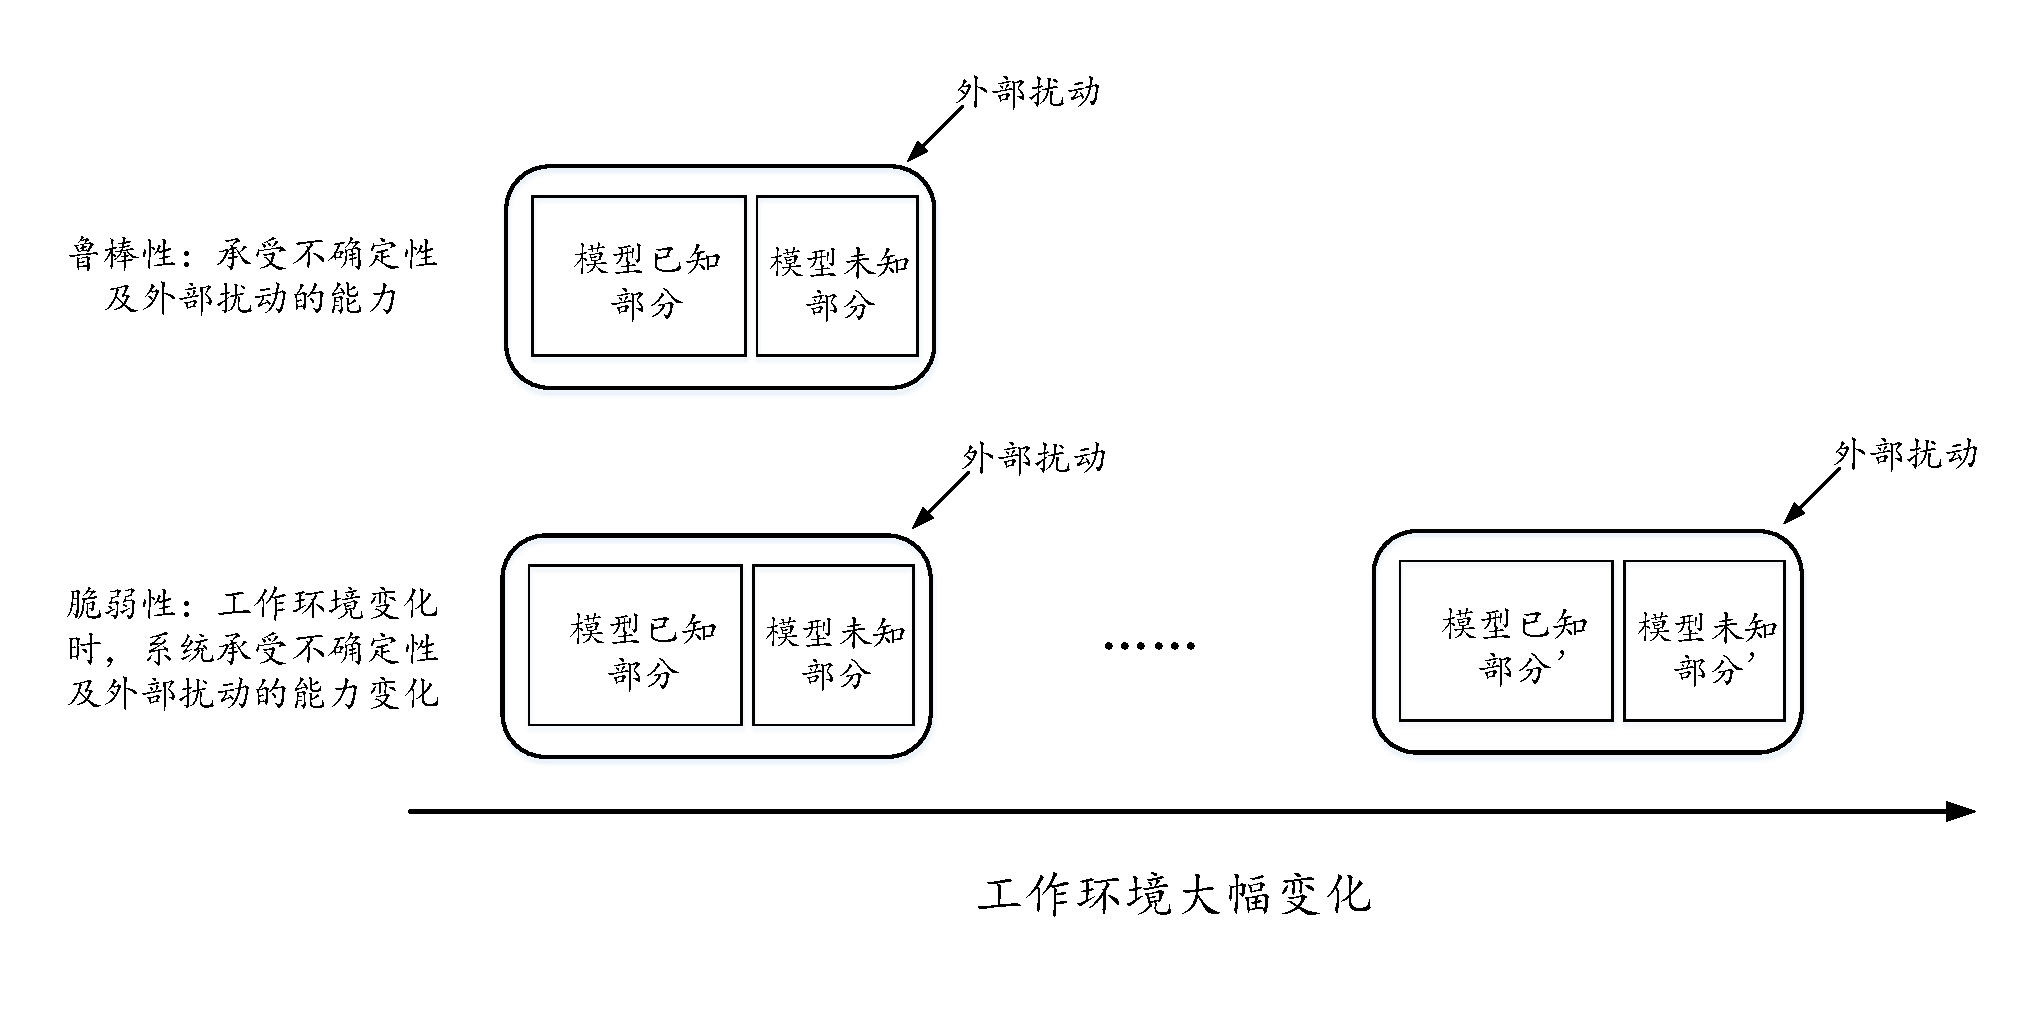
\includegraphics[width=14cm]{Robust.pdf}\\
   \caption{系统脆弱性与鲁棒性概念的区别}\label{fig:chap2:robust}
\end{figure}

综合上述对控制系统稳定性与鲁棒性的分析以及对脆弱性问题本质的探究,本文中对控制系统的脆弱性做如下定义:

当控制系统已知部分参数由于工作环境变化而发生了改变,系统承受不确定性的能力迅速变差,这种隐性的系统性能即为控制系统的脆弱性。

\section{控制系统灵敏度分析}
\label{sec:chap3:ControlSystem_Sensitivity}
控制系统的脆弱性表现为系统能承受不确定性能力的变坏程度,因此不确定性即为控制系统具有脆弱性这种隐性性能的本质原因。采用数学方式对控制系统脆弱性问题进行描述,首先需要对控制系统的不确定性进行分析与量化,然后采用控制理论及鲁棒控制理论中的相关知识对控制系统脆弱性问题进行科学的数学描述。
\subsection{控制系统的不确定性}
对于现实世界中的控制对象,几乎无法建立完美精确的数学模型,在建模的过程中都会进行一定程度上的工程近似处理,这些对实际问题的工程近似处理导致了控制对象数学模型的不确定性。由于控制系统数学模型在建模时将实际参数理想化,并未考虑被控对象、控制器、执行机构以及反馈机构的实际物理参数变化。因此,当工作环境的变化导致控制系统实际物理参数发生变化时,系统容易出现数学模型的不确定性。系统的不确定性主要可分为三类:结构不确定性、非结构不确定性以及混合不确定性。

~(1)~结构不确定性

系统的结构不确定性主要指控制系统中某些参数值是在一定的参数集合中取值而不是确定的参数值。这种类型的不确定性也称为结构性摄动,这种摄动仅影响系统的参数而不影响系统模型的结构,即在一定的系统模型结构中参数的不确定性。

结构不确定性主要来源于参数的测量误差、参数的实际值与标称值误差、环境和运行条件的变化这三个方面。由于测量技术的限制,控制系统中许多参数的测量值会存在一定的误差,尤其是在热力学、流体力学及空气动力学问题中,很难做到参数的精确测量。这些系统参数的测量误差,是结构不确定性产生的原因之一\cite{Yang2000UncertaintyControl}。

环境及运行条件的变化也是结构不确定性产生的重要原因。控制系统内部物理元件老化导致元件参数的变化,直接导致控制系统模型参数的变化。例如电路系统工作环境温度急剧变化,电子元器件参数会根据温度变化而产生漂移;飞机和导弹在高空或低空以高速或低速飞行时,相应的空气动力学参数会发生剧烈的变化,甚至由于燃料消耗造成的导弹质量与质心的变化,都会改变控制系统的模型参数,从而导致系统结构不确定性\cite{Keel2010Control,Zhao2016FlightControl}。

~(2)~非结构不确定性

系统的非结构不确定性主要指表现在系统结构上的不确定性,主要来源于系统模型辨识误差、系统工况变动影响、工程建模近似简化这三方面。针对一些机理不明确或机理特别复杂的控制系统,在工程实际中主要采用系统辨识的方式来建立系统的数学模型。然而,系统辨识的建模方法首先需要拟定系统模型的阶次,通过所建立模型的输出误差来判断辨识出模型的科学性。这就会导致由系统辨识方法建立的数学模型在低频中有很好的系统性能,但在高频段中系统性能会大幅变差,导致非结构不确定性\cite{Hu2001Uncertainty}。

系统工况变动也是导致系统非结构不确定性的一个原因。在分析实际工程问题时,常会遇到非线性的控制对象。在建立数学模型时,需要针对控制系统的静态工作点进行分析,对控制系统静态工作点处进行线性化建模。如果被控对象的工作点偏离静态工作点,控制系统的数学模型就会与实际的模型产生偏差,从而产生非结构不确定性。

~(3)~混合不确定性

实际工程问题中,建模的方式并不唯一。参数的测量误差普遍存在,至今仍有许多优秀的科学家及工程师尝试研制更高精度的测量系统以及更精确的测量仪器。系统的数学模型或多或少会存在结构不确定性,而系统辨识、线性化建模及工程近似简化也是系统建模的常用方式,因此建立控制系统的数学模型中常常会同时包含结构不确定性及非结构不确定性,这种系统则具有混合不确定性。
\subsection{反馈控制系统的性能}
反馈是现代控制理论中的核心概念,绝大多数控制系统都是基于反馈概念设计的。通过合理地设置反馈,控制系统的输出能够良好地跟随参考输入信号,并且能够有效抑制外部扰动及测量误差信号对控制系统产生的影响。在分析控制系统脆弱性之前,首先分析反馈对系统的作用,然后基于反馈对系统性能的影响将系统脆弱性问题转化为数学问题进行分析。

反馈控制系统的各方面性能是设计与分析控制系统的主要关注点,对于一个简单的闭环反馈控制系统,控制框图如图~\ref{fig:chap2:feedback1}~所示。
\begin{figure}[h]
  \centering
     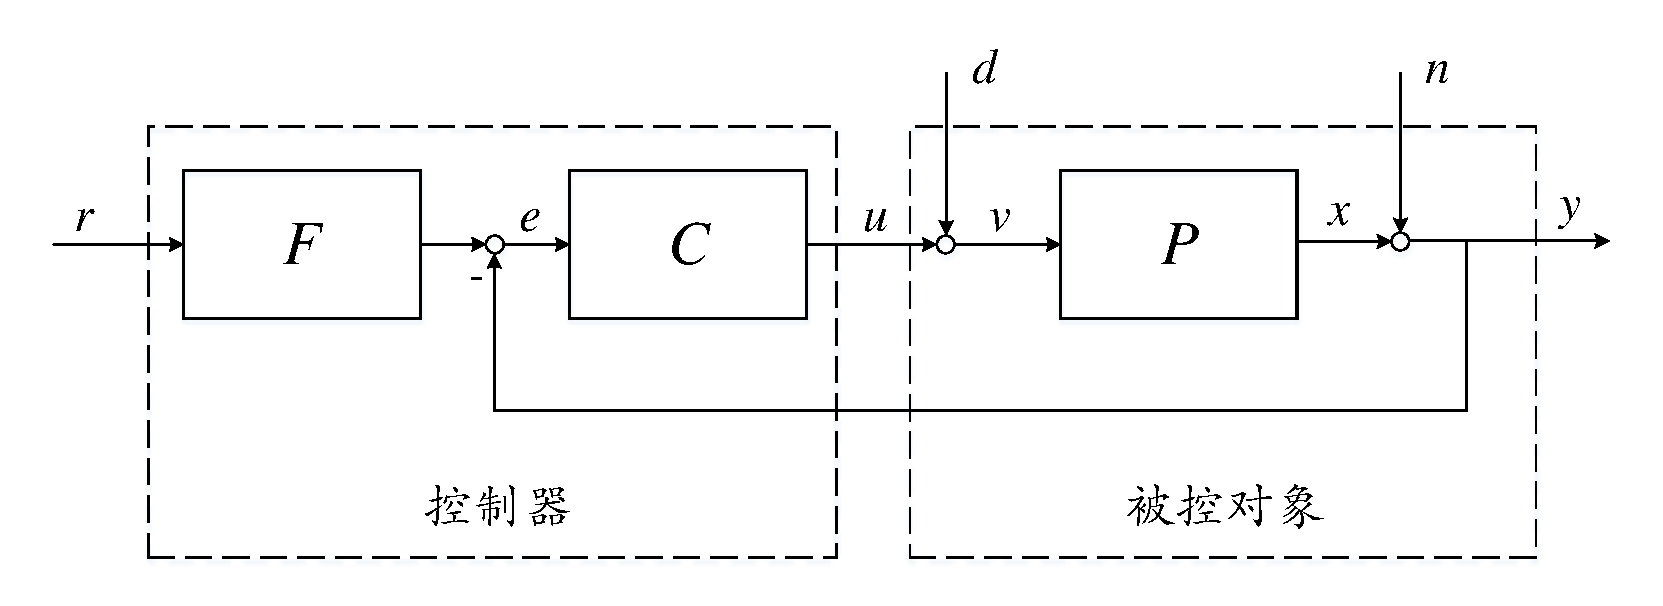
\includegraphics[width=11cm]{Feedback1.pdf}\\
   \caption{闭环反馈系统控制框图}\label{fig:chap2:feedback1}
\end{figure}

闭环控制系统是由两部分组成的,被控对象与控制器。其中,控制器也是由两部分所构成的,分别是前馈控制器~F~与反馈控制器~C。对于被控对象部分,负载扰动~d~与测量误差扰动~n~会对系统产生影响。在系统工作过程中,被控对象的工作状态常会由于外部环境的干扰及自身不确定性的影响而发生变化,这些扰动在闭环反馈系统控制框图中采用负载扰动~d~来代表。控制器是基于被控对象控制参数的检测值而工作的,由于反馈参数的测量误差是客观存在的,因此测量误差信号~n~作为扰动输入到系统当中。为使控制系统脱离结构的束缚,更好地关注控制系统各个信号之间本质的关系,将图~\ref{fig:chap2:feedback1}~所示的反馈控制系统归纳简化为图~\ref{fig:chap2:feedback2}~所示的最一般的控制系统框图。
\begin{figure}[h]
  \centering
     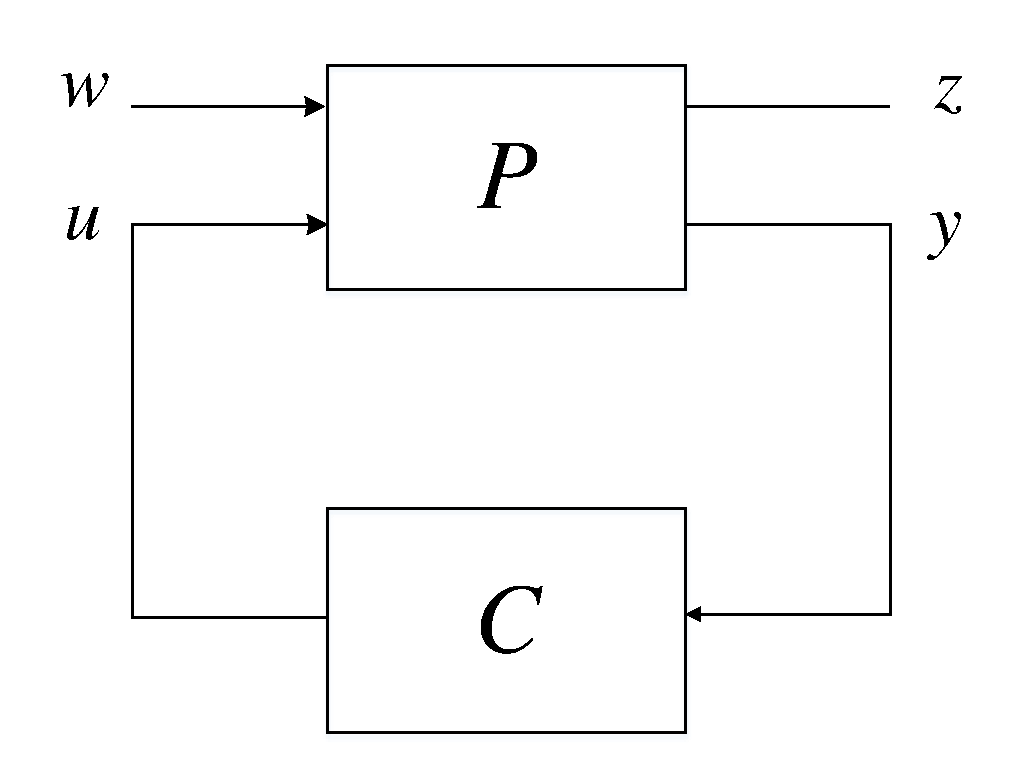
\includegraphics[width=5.5cm]{Feedback2.pdf}\\
   \caption{一般的控制系统}\label{fig:chap2:feedback2}
\end{figure}

在图~\ref{fig:chap2:feedback2}~中输入信号被分为两类,一类为控制信号~u,另一类为外部扰动对控制系统产生的影响~w=(r, d, n)。输出信号也分为两类,一类为检测信号~y,另一类为其他信号~z=(e, v, x)。被控对象~P~为实际控制对象集合,即执行机构、传感器、A/D~和~D/A~转换器件等。控制器部分~C~为控制系统可设计的部分,即电子电路、可编程控制器、工业控制计算机或其他控制装置。

在分析与设计反馈控制系统时,通常需要考虑以下~5~个方面:

(1)~系统的稳定性

(2)~系统对参考输入信号的跟随能力

(3)~系统对负载扰动的抑制能力

(4)~系统对测量误差干扰的抑制能力

(5)~系统对模型不确定性的抑制能力

其中,稳定性是控制系统正常工作的前提条件,而后面四个为控制系统的重要性能指标。针对不同的实际工作情况,设计控制系统时的侧重有所不同。对于随动系统,系统的输出量随输入量的变化而变化。因此设计随动系统时,应着重关注系统对参考输入信号的跟随能力及定位的准确性。在其他控制系统中,抑制扰动的能力及系统的鲁棒性是主要关注的性能指标。

图~\ref{fig:chap2:feedback1}~描述的反馈控制系统有三个外部输入信号:参考输入信号~r、负载扰动信号~d~以及测量误差扰动信号~n。也有三个输出信号:控制器输出控制信号~u、被控对象的输出信号~x~与~y。分析这六个信号之间的相互关系是研究控制系统各方面性能的重要途径。因此,在分析反馈控制系统的性能时,首先将控制系统线性化,然后采用传递函数的方式来分析系统三个输入信号与三个输出信号之间的数学关系,从而研究系统的性能。

对控制系统输入输出信号进行拉普拉斯变换,根据叠加原理可以得到~X(s)、Y(s)、U(s)、D(s)、N(s)、R(s)~六个信号之间的关系式。

\begin{footnotesize}
\begin{equation}\label{equ:chap3:Index1}
\begin{aligned}
   &   X\left(s\right)=\FS{P\left(s\right)}{1+P\left(s\right)\cdot C\left(s\right)}\cdot D\left(s\right)-\FS{P\left(s\right)\cdot C\left(s\right) }{1+P\left(s\right)\cdot C\left(s\right)}\cdot N\left(s\right)+\FS{P\left(s\right)\cdot C\left(s\right)\cdot F\left(s\right) }{1+P\left(s\right)\cdot C\left(s\right)}\cdot R\left(s\right) \\
   &   Y\left(s\right)=\FS{P\left(s\right)}{1+P\left(s\right)\cdot C\left(s\right)}\cdot D\left(s\right)+\FS{1}{1+P\left(s\right)\cdot C\left(s\right)}\cdot N\left(s\right)+\FS{P\left(s\right)\cdot C\left(s\right)\cdot F\left(s\right) }{1+P\left(s\right)\cdot C\left(s\right)}\cdot R\left(s\right) \\
   &   U\left(s\right)=\FS{P\left(s\right)\cdot C\left(s\right)}{1+P\left(s\right)\cdot C\left(s\right)}\cdot D\left(s\right)-\FS{C\left(s\right)}{1+P\left(s\right)\cdot C\left(s\right)}\cdot N\left(s\right)+\FS{C\left(s\right)\cdot F\left(s\right) }{1+P\left(s\right)\cdot C\left(s\right)}\cdot R\left(s\right) \\
\end{aligned}
\end{equation}
\end{footnotesize}

通过分析式~\ref{equ:chap3:Index1}~的三个等式可知,控制系统的 三个输入信号~R(s)、N(s)、D(s)~与三个输出信号~X(s)、Y(s)、U(s)~之间的数学关系是由以下~6~个函数所构成的。

\begin{table}[htbp]
\centering
\renewcommand\arraystretch{2}                                %表格高度为原来的两倍
      \begin{tabular}{C{3cm}C{3cm}C{3cm}}
                   $\FS{P\left(s\right)\cdot C\left(s\right)\cdot F\left(s\right)}{1+P\left(s\right)\cdot C\left(s\right)}$
               & $\FS{P\left(s\right)\cdot C\left(s\right)}{1+P\left(s\right)\cdot \left(s\right)}$
               &$\FS{P\left(s\right)}{1+P\left(s\right)\cdot C\left(s\right)}$\\

                   $\FS{C\left(s\right)\cdot F\left(s\right)}{1+P\left(s\right)\cdot C\left(s\right)}$
               & $\FS{C\left(s\right)}{1+P\left(s\right)\cdot C\left(s\right)}$
               & $\FS{1}{1+P\left(s\right)\cdot C\left(s\right)}$
\end{tabular}
\end{table}

从输入参考信号~R(s)~的角度来看,函数~\begin{footnotesize}$\FS{P\left(s\right)\cdot C\left(s\right)\cdot F\left(s\right)}{1+P\left(s\right)\cdot C\left(s\right)}$\end{footnotesize}~反映的是参考输入信号~R(s)~对被控对象输出信号~X(s)~与~Y(s)~的影响;函数~\begin{footnotesize}$\FS{C\left(s\right)\cdot F\left(s\right)}{1+P\left(s\right)\cdot C\left(s\right)}$\end{footnotesize}~反映的是参考输入信号~R(s)~对控制器输出控制信号~U(s)~的影响。

对于纯反馈~(pure feedback)~控制系统,前馈控制器环节的拉普拉斯变换~F(s)~为~1,系统的所有控制效果都是由反馈控制器实现的,则纯反馈控制系统的输入与输出信号之间的数学关系为

\begin{footnotesize}
\begin{equation}\label{equ:chap3:Index2}
\begin{aligned}
   &   X\left(s\right)=\FS{P\left(s\right)}{1+P\left(s\right)\cdot C\left(s\right)}\cdot D\left(s\right)-\FS{P\left(s\right)\cdot C\left(s\right) }{1+P\left(s\right)\cdot C\left(s\right)}\cdot N\left(s\right)+\FS{P\left(s\right)\cdot C\left(s\right) }{1+P\left(s\right)\cdot C\left(s\right)}\cdot R\left(s\right) \\
   &   Y\left(s\right)=\FS{P\left(s\right)}{1+P\left(s\right)\cdot C\left(s\right)}\cdot D\left(s\right)+\FS{1}{1+P\left(s\right)\cdot C\left(s\right)}\cdot N\left(s\right)+\FS{P\left(s\right)\cdot C\left(s\right)}{1+P\left(s\right)\cdot C\left(s\right)}\cdot R\left(s\right) \\
   &   U\left(s\right)=\FS{P\left(s\right)\cdot C\left(s\right)}{1+P\left(s\right)\cdot C\left(s\right)}\cdot D\left(s\right)-\FS{C\left(s\right)}{1+P\left(s\right)\cdot C\left(s\right)}\cdot N\left(s\right)+\FS{C\left(s\right)}{1+P\left(s\right)\cdot C\left(s\right)}\cdot R\left(s\right) \\
\end{aligned}
\end{equation}
\end{footnotesize}

由式~\ref{equ:chap3:Index2}~所示的三个等式可知,纯反馈控制系统的输入与输出信号之间的数学关系可以由~4~个函数来描述。通过研究这四个函数的特性,分析纯反馈控制系统对参考输入信号的跟随能力、对负载扰动的抑制能力、对测量误差扰动的抑制能力等重要系统性能。

\medskip
 \begin{small}$\FS{P\left(s\right)\cdot C\left(s\right)}{1+P\left(s\right)\cdot \left(s\right)}$ \end{small},~~补灵敏度函数

 \medskip
 \begin{small}$\FS{P\left(s\right)}{1+P\left(s\right)\cdot C\left(s\right)}$\end{small},负载扰动灵敏度函数

 \medskip
 \begin{small}$\FS{C\left(s\right)}{1+P\left(s\right)\cdot C\left(s\right)}$\end{small},测量误差扰动灵敏度函数

  \medskip
 \begin{small}$\FS{1}{1+P\left(s\right)\cdot C\left(s\right)}$\end{small},灵敏度函数
 \subsection{控制系统灵敏度的数学描述}
 在工程领域中,分析与设计控制系统灵敏度函数是研究控制系统性能的常用方式。由上一节中分析可知,系统对负载扰动及测量误差扰动的灵敏度函数都可由系统灵敏度函数转换得到,且很多控制系统性能往往都可以用灵敏度函数和补灵敏度函数来表示。

 在分析控制系统灵敏度函数对系统性能的影响之前,首先定义灵敏度函数这一概念。考虑一个依赖于参数~$x_1,x_2,...,x_n$~的函数~$f(x_1,x_2,...,x_n)$,当参数~$x_i$~发生变化时,若函数~$f$~的值变化很大,则称函数~$f$~对参数~$x_i$~的灵敏度大。若当参数~ $x_i$~发生变化时,函数~$f$~的值没有发生较大的变化,则称函数~$f$~对参数~ $x_i$~的灵敏度小。将参数~ $x_i$~的变化记为~$\Delta x_i$,则函数~$f$~的变化为
 \begin{equation}\label{equ:chap3:Index3}
  \Delta_i f\left(x_1,x_2,...,x_n\right)=f\left(x_1,x_2,...,x_i+\Delta x_i,...,x_n\right)-f\left(x_1,x_2,...,x_i,...,x_n\right)
\end{equation}

依据对灵敏度函数的语义分析,可以将灵敏度函数表示为
 \begin{equation}\label{equ:chap3:Index4}
\hat{S}_{x_i}=\FS{\Delta_i f(x_1,x_2,...,x_n)/f(x_1,x_2,...,x_n)}{\Delta x_i/x_i}
\end{equation}

由于灵敏度函数强调的是参数的微小变化对函数~$f$~的影响程度,因此实际灵敏度函数的表达式为
\begin{equation}\label{equ:chap3:Index5}
   S_{x_i}=\lim_{\Delta x_i \to 0}\FS{\Delta_i f(x_1,x_2,...,x_n)/f(x_1,x_2,...,x_n)}{\Delta x_i/x_i}=\FS{df(x_1,x_2,...,x_n)}{dx_i}\cdot \FS{x_i}{f(x_1,x_2,...,x_n)}
\end{equation}

对于控制系统的灵敏度函数有不同的分析方法,本文从控制系统模型不确定性和控制系统反馈环节的作用这两个不同的角度来进行分析。

~(1)~控制系统模型的不确定性

在纯反馈控制系统中,当负载扰动~D~与测量误差扰动信号~N~为~0~时,反馈系统的闭环传递函数为
\begin{equation}\label{equ:chap3:Index6}
  T\left(s\right)=\FS{P\left(s\right)\cdot C\left(s\right)}{1+P\left(s\right)\cdot C\left(s\right)}
\end{equation}

若由于系统存在不确定性,即被控对象的模型~P(s)~不是精确的数学模型,则可以把~P(s)~作为变化的参数来分析计算传递函数~T(s)~对参数~P(s)~变化的灵敏度函数。记被控对象数学模型的变化为~$P\left(s\right)+\Delta P\left(s\right)$  ,闭环系统传递函数的变化~$\Delta T\left(s\right)$~为
\begin{equation}\label{equ:chap3:Index7}
 \begin{aligned}
  \Delta T\left(s\right)&=\FS{\left[P\left(s\right)+\Delta P\left(s\right)\right]\cdot C\left(s\right)}{1+\left[P\left(s\right)+\Delta P\left(s\right)\right]\cdot C\left(s\right)}-\FS{P\left(s\right)\cdot C\left(s\right)}{1+P\left(s\right)\cdot C\left(s\right)}\\
  &=\FS{\Delta P\left(s\right)\cdot C\left(s\right)}{\left\{1+\left[P\left(s\right)+\Delta P\left(s\right)\right]\cdot C\left(s\right)\right\}}\cdot \left[1+P\left(s\right)\cdot C\left(s\right)\right]\\
  &=\FS{\Delta P\left(s\right)}{1+\left[P\left(s\right)+\Delta P\left(s\right)\right]\cdot C\left(s\right)}\cdot \FS{T\left(s\right)}{P\left(s\right)}
  \end{aligned}
\end{equation}

传递函数~T(s)~对参数~P(s)~变化的灵敏度函数为
\begin{small}
\begin{equation}\label{equ:chap3:Index8}
     S_{T\left(s\right)}=\lim_{\Delta P\left(s\right) \to 0}\FS{\Delta T\left(s\right)/T\left(s\right)}{\Delta P\left(s\right)/P\left(s\right)}=\lim_{\Delta P\left(s\right) \to 0}\FS{1}{1+\left[P\left(s\right)+\Delta P\left(s\right)\cdot C\left(s\right)\right]}=\FS{1}{1+P\left(s\right)\cdot C\left(s\right)}
\end{equation}
\end{small}

传递函数~T(s)~也称为补灵敏度函数
\begin{equation}\label{equ:chap3:Index9}
  T\left(s\right)=1-S_{T\left(s\right)}=\FS{P\left(s\right)\cdot C\left(s\right)}{1+P\left(s\right)\cdot C\left(s\right)}
\end{equation}

从控制系统模型不确定性的角度来分析,灵敏度函数表征的是系统模型不确定的微小变化对系统闭环传递函数的影响程度。

~(2)~控制系统反馈环节的作用

从控制系统反馈环节的角度来看,灵敏度函数表征的是反馈环节对系统的作用。如图~\ref{fig:chap2:openl_closel}~所示的开环与闭环系统控制框图,可得系统开环传递函数~$Y_{ol}(s)$~与闭环传递函数~$Y_{cl}(s)$~之间的数学关系为
\begin{equation}\label{equ:chap3:Index10}
  Y_{cl}(s)=\FS{1}{1+P\left(s\right)\cdot C\left(s\right)}\cdot Y_{ol}\left(s\right)=S\left(s\right)\cdot Y_{ol}\left(s\right)
\end{equation}

相比于开环控制系统,闭环反馈控制系统的作用在于将开环传递函数的输出信号通过灵敏度函数矫正后再输出,这正是反馈环节对控制系统的作用。在闭环反馈系统中,负载扰动信号~D~与测量误差扰动信号~N~都经过灵敏度函数~$S\left(s\right)$~的矫正,且不同工作频率下灵敏度函数对扰动信号有不同的矫正作用。

当灵敏度函数的幅值在工作频率范围内满足~$\left\vert S\left(jw\right)\right\vert<1$,则灵敏度函数~$S\left(s\right)$~对负载扰动信号~D~与测量误差扰动信号~N~产生抑制作用。当灵敏度函数的幅值在工作频率范围内满足~$\left\vert S\left(jw\right)\right\vert>1$,则灵敏度函数~$S\left(s\right)$~对负载扰动信号与测量误差扰动信号起到放大作用。灵敏度函数幅值的最大值为~$M_s$,对应的系统频率记为~$w_{ms}$。
\begin{equation}\label{equ:chap3:Index11}
  M_s=\max\limits_{w}\left\vert S\left(jw\right)\right\vert=\left\vert\FS{1}{1+P\left(jw_{ms}\right)\cdot C\left(jw_{ms}\right)}\right\vert
\end{equation}

\begin{figure}[h]
  \centering
     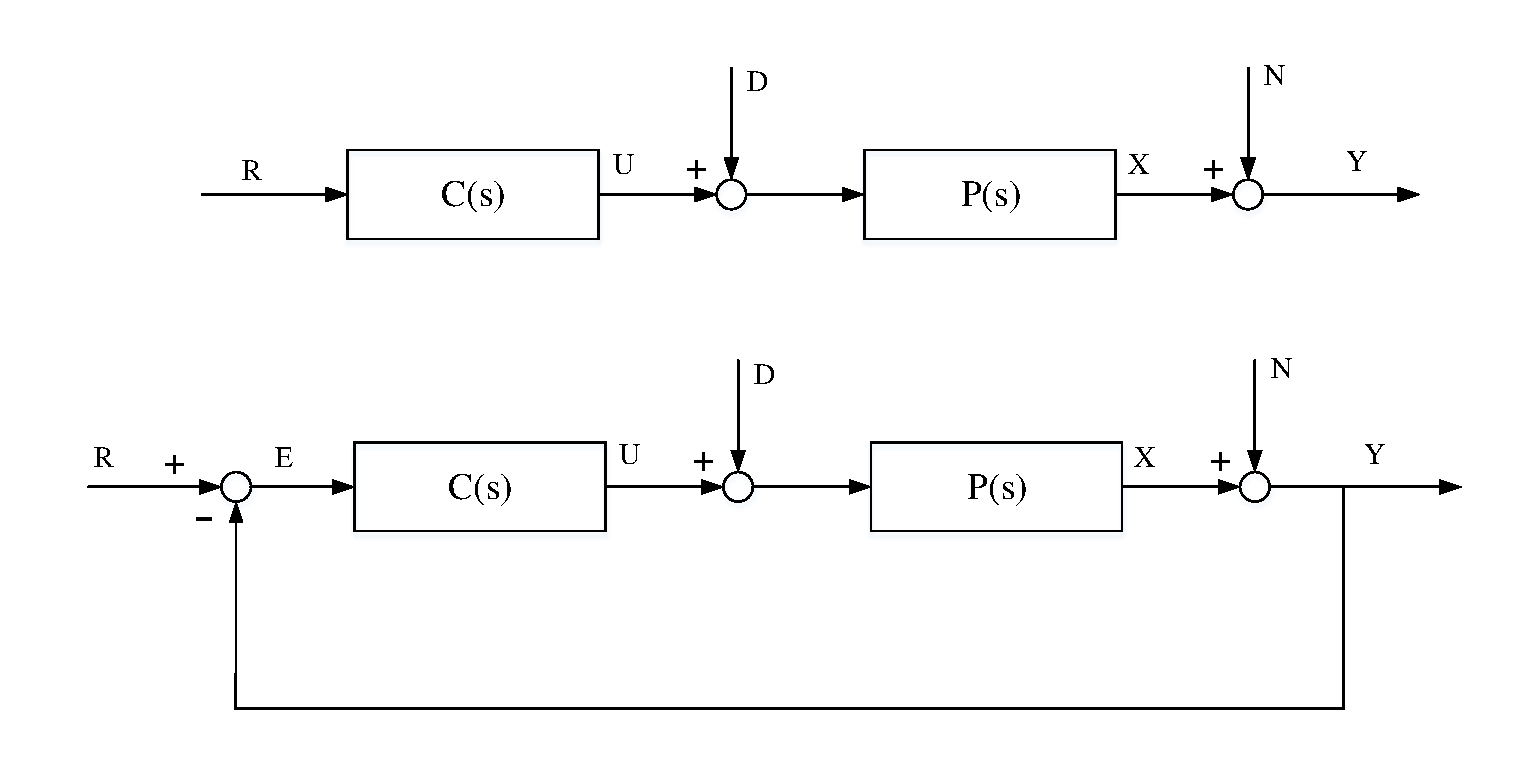
\includegraphics[width=11cm]{OpenL_CloseL.pdf}\\
   \caption{开环与闭环系统控制框图}\label{fig:chap2:openl_closel}
\end{figure}
\begin{figure}[h]
  \centering
     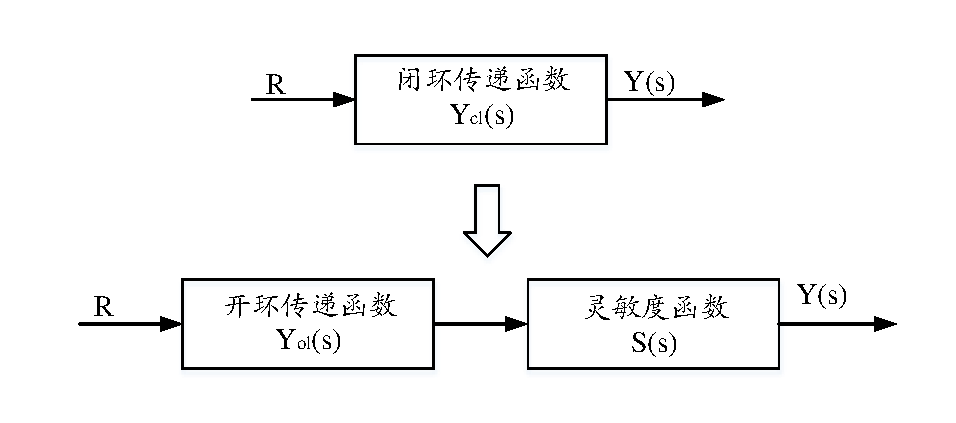
\includegraphics[width=11cm]{SensibilityFunction.pdf}\\
   \caption{灵敏度函数的作用}\label{fig:chap2:sensibilityfunction}
\end{figure}

%当灵敏度函数的幅值~$\left\vert S\left(jw\right)\right\vert$~大于~1~时,反馈系统对负载扰动信号与测量误差扰动信号起到放大作用,灵敏度函数幅值的最大值为~$M_s$,对应的系统频率记为~$w_{ms}$。


对于确定的反馈控制系统,可以通过灵敏度函数的~Bode~图来分析反馈控制器对系统扰动信号的抑制作用。以比例积分控制器为例,开环传递函数为
\begin{equation}\label{equ:chap3:Index12}
  C\left(s\right)\cdot P\left(s\right)=\FS{10}{s\cdot \left(s+1\right)}
\end{equation}

灵敏度函数~S(s)~为
\begin{equation}\label{equ:chap3:Index13}
  S\left(s\right)=\FS{1}{1+C\left(s\right)\cdot P\left(s\right)}=\FS{s\cdot \left(s+1\right)}{s\cdot \left(s+1\right)+10}
\end{equation}

由于灵敏度函数~S(s)~可以写成
\begin{equation}\label{equ:chap3:Index14}
  S\left(s\right)=\FS{1}{1+C\left(s\right)\cdot P\left(s\right)}=\FS{1}{1+L\left(s\right)}
\end{equation}

由图~\ref{fig:chap3:Bodegraph}~所示灵敏度函数~S(s)~的~Bode~图可知,最大灵敏度~\begin{small}$M_s=10.5dB=3.35$\end{small},对应的系统频率为~0.52Hz,系统频率~0.356Hz~对应的灵敏度函数幅值为~\begin{small}$\left\vert S\left(jw\right)\right\vert=0dB=1$\end{small}。通过分析灵敏度函数曲线可知,在频率低于~0.356Hz~时,比例积分控制系统对负载扰动及测量误差扰动起到抑制作用,当频率高于~0.356Hz~时,系统对负载扰动及测量误差扰动起到放大作用,最大放大倍数为~3.35~倍。

\begin{figure}[h]
  \centering
     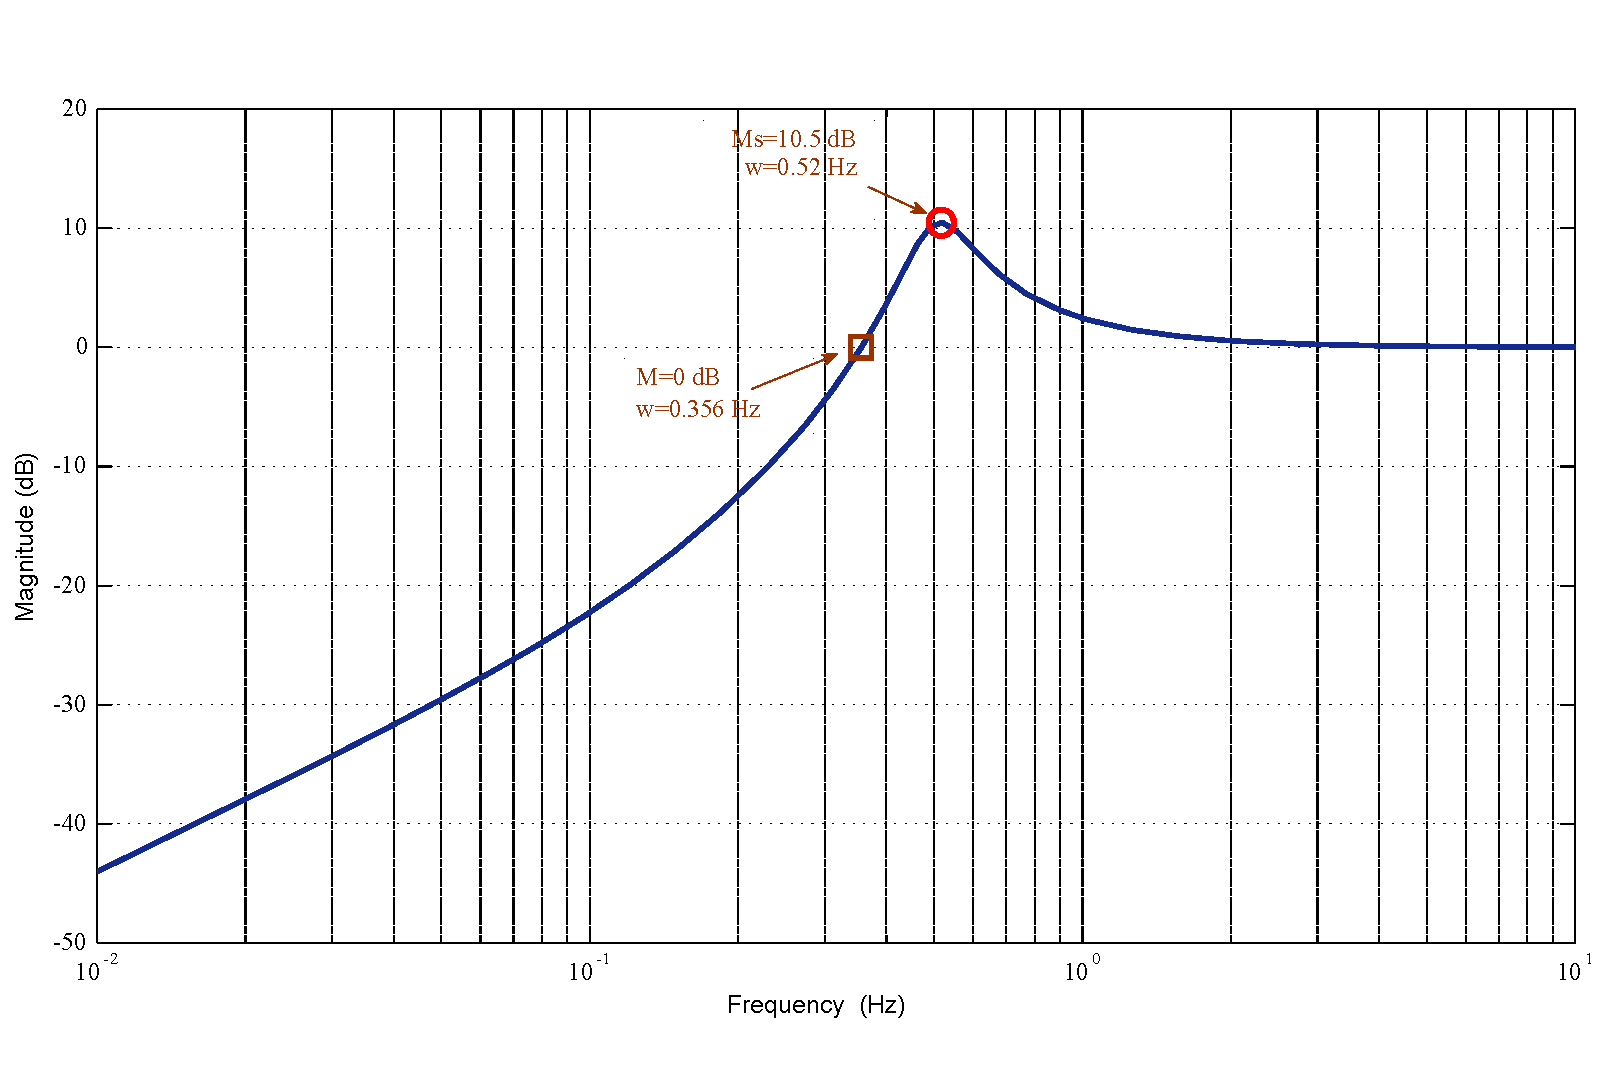
\includegraphics[width=14cm]{NEWBG.pdf}
   \caption{比例积分控制系统灵敏度函数的~Bode~图}\label{fig:chap3:Bodegraph}
\end{figure}

在复平面内,可以将复数~$1+L\left(jw\right)$~看作由~(-1,~j0)~点指向奈奎斯特曲线上~$L\left(jw\right)$~点的向量,则向量的模为~$\left\vert1+L\left(jw\right)\right\vert$。从奈奎斯特曲线的角度来看灵敏度函数的幅值即为从~(-1,~j0)~点指向奈奎斯特曲线上 点~$L\left(jw\right)$~的向量模的倒数。因此如图~\ref{fig:chap3:sensitivitygraph}~所示,以~(-1,~j0)~点为圆心画一个半径为~1~的圆,奈奎斯特曲线中在圆内的点对应灵敏度函数的幅值~$\left\vert S\left(jw\right)\right\vert$~大于~1,反馈系统对负载扰动信号与测量误差扰动信号起到放大作用,而在圆外的点对应灵敏度函数的幅值~$\left\vert S\left(jw\right)\right\vert$~小于1,反馈系统对负载扰动信号与测量误差扰动信号起到抑制作用。灵敏度函数幅值的最大值~$M_s$~为系统奈奎斯特曲线与~(-1,~j0)~点最短距离的倒数。
\begin{figure}[h]
  \centering
     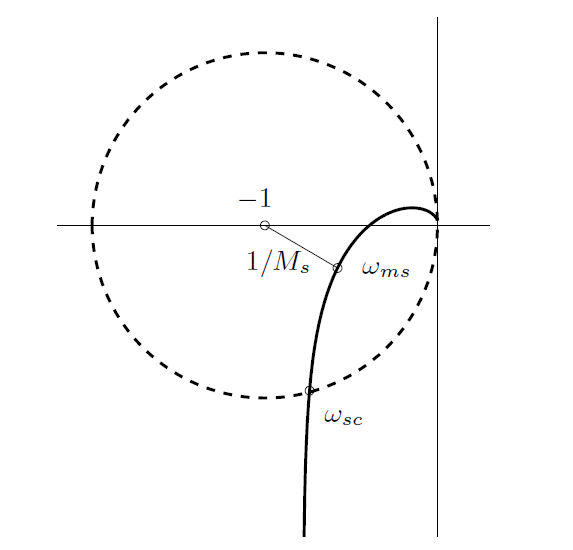
\includegraphics[width=7.5cm]{SensitivityGraph.png}\\
   \caption{灵敏度函数与奈奎斯特曲线}\label{fig:chap3:sensitivitygraph}
\end{figure}

\section{控制系统脆弱性问题的数学描述}
\label{sec:chap3:Fragility_Math}
根据上文对控制系统脆弱性概念的分析与定义可知,研究控制系统的脆弱性问题即为研究系统承受不确定性能力的变化趋势。由~3.3.1~节对系统不确定性的产生原因及分类可知,系统不确定性可分为结构不确定性与非结构不确定性。相比结构不确定性,对控制系统非结构不确定性的分析与描述更加重要,因为工程实际控制系统中采用的控制对象模型普遍具有未建模部分,需要分析与描述控制系统在某种界限范围内的所有不确定性,并研究未建模不确定部分的动态特性。因此,本文基于控制系统非结构不确定性来研究系统的脆弱性。

系统的非结构不确定性有两种数学描述方式:加性不确定性与乘性不确定性。加性不确定性将实际控制对象的传递函数~$P_A\left(s\right)$~与标称模型的传递函数~$P\left(s\right)$~之差~$P_A\left(s\right)-P\left(s\right)$~作为系统的不确定性,数学描述为
\begin{equation}\label{equ:chap3:Index15}
  P_A\left(s\right)=P\left(s\right)+\hat{\Delta} \left(s\right)
\end{equation}

乘性不确定性将实际控制对象的传递函数~$P_A\left(s\right)$~与标称模型的传递函数~$P\left(s\right)$~的相对差~\begin{small}$\left[P_A\left(s\right)-P\left(s\right)\right]\cdot P^{-1}\left(s\right)$\end{small}~作为系统不确定性,数学描述为
\begin{equation}\label{equ:chap3:Index16}
  P_A\left(s\right)=P\left(s\right)+\hat{\Delta} \left(s\right)\cdot P\left(s\right)
\end{equation}

由于系统的不确定性要在一定的界限范围内,因此系统不确定性满足式~\ref{equ:chap3:Index17}。
\begin{equation}\label{equ:chap3:Index17}
 \left\vert\hat{\Delta}\left(jw\right)\right\vert\leq \left\vert W\left(jw\right)\right\vert
\end{equation}

则系统的不确定性可以表示为
\begin{equation}\label{equ:chap3:Index18}
\hat{\Delta}\left(s\right)=\Delta\left(s\right)\cdot W\left(s\right)
\end{equation}

其中~$\left\vert\Delta\left(jw\right)\right\vert\leq 1$,加性不确定性与乘性不确定性的系统框图如下图所示。
\begin{figure}[h]
\begin{minipage}[t]{0.5\linewidth}
  \centering
  % Requires \usepackage{graphicx}
  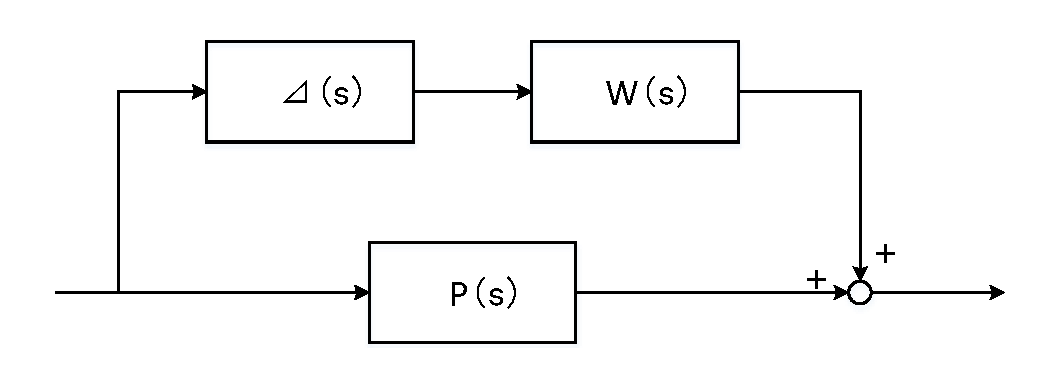
\includegraphics[width=7cm]{AddUnc.pdf}\\
  \caption{加性不确定性系统结构图}\label{fig:chap3:addunc}
\end{minipage}
\begin{minipage}[t]{0.5\linewidth}
  \centering
  % Requires \usepackage{graphicx}
  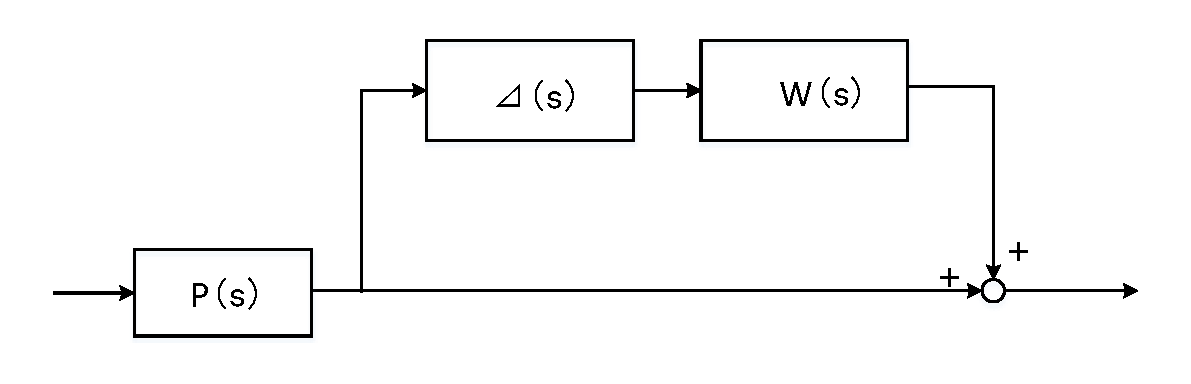
\includegraphics[width=7cm]{TimeUnc.pdf}\\
  \caption{乘性不确定性系统结构图}\label{fig:chap3:timeunc}
\end{minipage}
%\caption{非结构不确定性系统结构图}
\end{figure}

以上两种非结构不确定描述方法的主要区别在于:加性不确定性描述的是控制对象数学模型的绝对误差,而乘性不确定性描述的是控制对象数学模型的相对误差。在分析与研究控制系统脆弱性时,主要考虑的是模型绝对误差给系统带来的影响。因此,以系统加性不确定性的方式对系统模型未建模部分进行描述,在此基础上分析控制系统的脆弱性。

具有加性不确定性的反馈控制系统结构图如图~\ref{equ:chap3:Index19}~所示,标称开环传递函数为
\begin{equation}\label{equ:chap3:Index19}
L_o\left(s\right)=C\left(s\right)\cdot P\left(s\right)
\end{equation}

具有加性不确定性的实际开环传递函数为
\begin{equation}\label{equ:chap3:Index20}
L_A\left(s\right)=C\left(s\right)\cdot P\left(s\right)+C\left(s\right)\cdot \Delta\left(s\right)\cdot W\left(s\right)
\end{equation}
\begin{figure}[h]
  \centering
     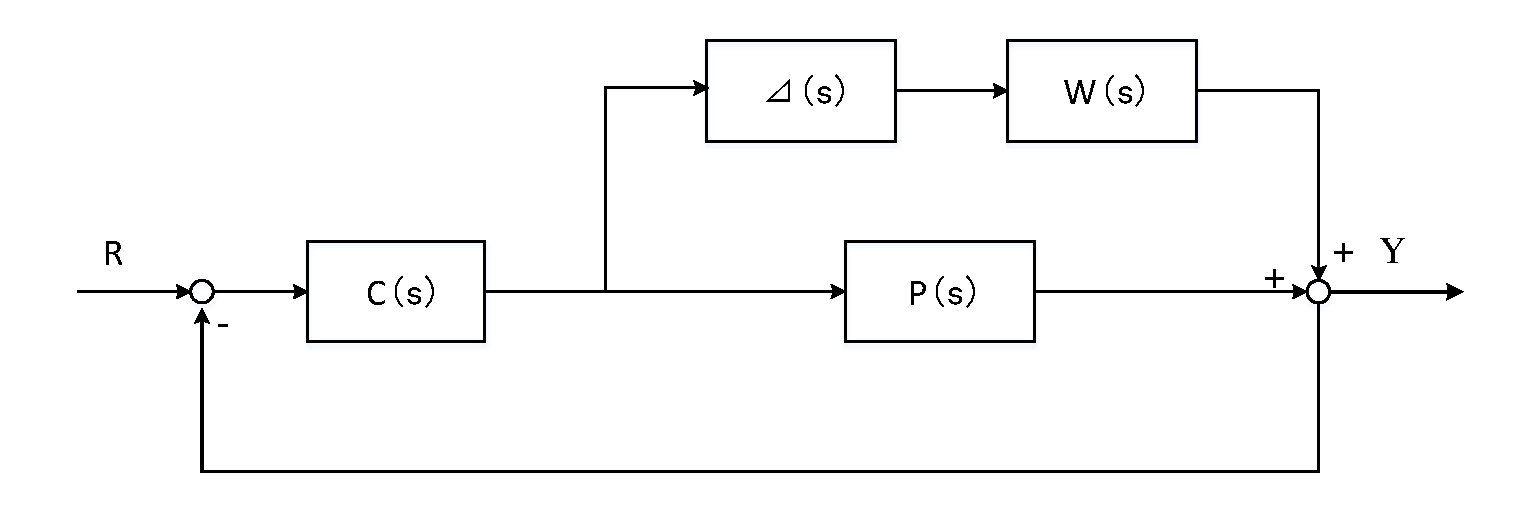
\includegraphics[width=12cm]{Con_AddUnc.pdf}\\
   \caption{具有加性不确定性的系统结构图}\label{fig:chap3:conaddunc}
\end{figure}

保持稳定工作是控制系统最重要的性能指标,脆弱性研究的主要问题是系统稳定工作时容忍不确定性能力的变化趋势。从奈奎斯特图的角度来分析,式~\ref{equ:chap3:Index20}~可以写为
\begin{equation}\label{equ:chap3:Index21}
1+L_A\left(s\right)=1+C\left(s\right)\cdot P\left(s\right)+C\left(s\right)\cdot \Delta\left(s\right)\cdot W\left(s\right)=1+L_o\left(s\right)+C\left(s\right)\cdot \Delta\left(s\right)\cdot W\left(s\right)
\end{equation}

从复平面向量的角度来看,由于~$\left\vert\Delta\left(jw\right)\right\vert\leq 1$,所以~\begin{small}$C\left(s\right)\cdot\Delta\left(s\right)\cdot W\left(s\right)$\end{small}~代表的向量一定在以系统开环奈奎斯特曲线上点~$L_o\left(jw\right)$~为圆心,半径为~$\left\vert C\left(jw\right)\cdot W\left(jw\right)\right\vert$~的实心圆内,该实心圆即为不确定性对系统造成的影响在奈奎斯特图上的体现。如图~\ref{fig:chap3:nycurve1}~所示,A~点为~(-1,~j0)~点,B~点为系统标称开环传递函数当系统频率为~w~时的点,C~点为在加性不确定性影响下,系统实际开环传递函数频率为~w~时的点。为分析不确定性对系统造成的最大影响,C~点位于圆的边界上。由复平面向量的关系可知,式~\ref{equ:chap3:Index21}~表示的向量关系为
\begin{equation}\label{equ:chap3:Index22}
\overrightarrow{AC}=\overrightarrow{AB}+\overrightarrow{BC}
\end{equation}

由奈奎斯特定理可知,若控制系统开环传递函数的奈奎斯特曲线不包括~(-1,~j0)~点,则系统稳定。若系统在不确定性的影响下,实际开环传递函数的奈奎斯特曲线仍然不包括~(-1,~j0)~点,则系统能够容忍该不确定性并稳定工作。
\begin{figure}[h]
  \centering
     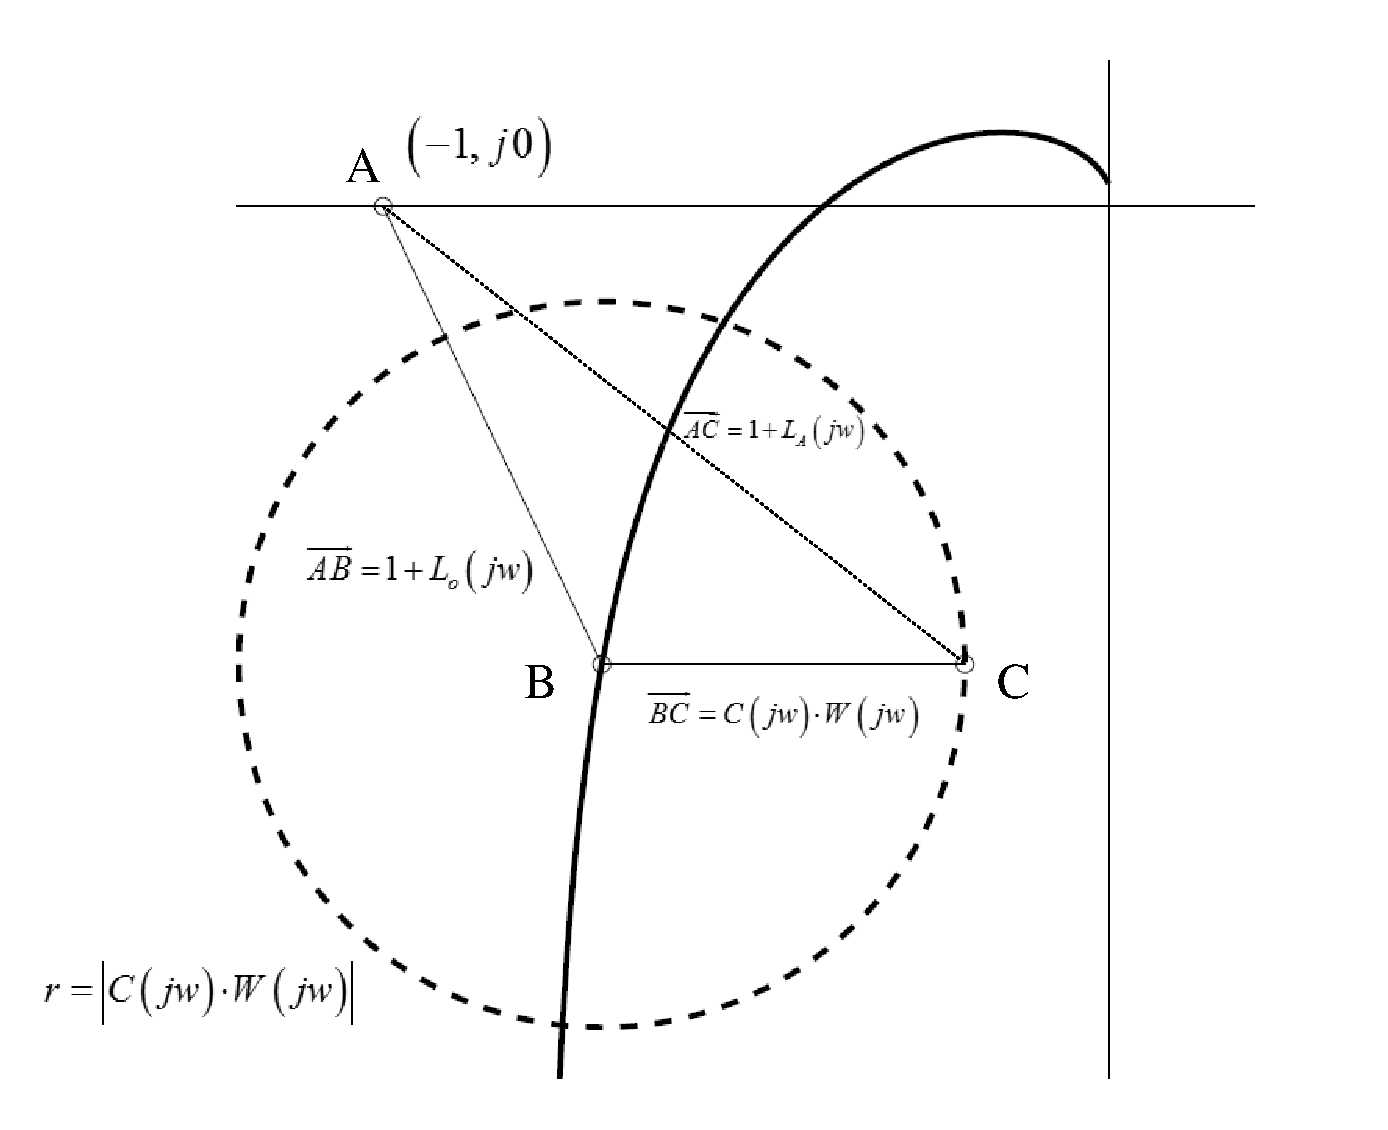
\includegraphics[width=10cm]{NyCurve1.pdf}\\
   \caption{具有不确定性系统的奈奎斯特图}\label{fig:chap3:nycurve1}
\end{figure}

为保证系统在不确定性的影响下可以稳定工作,则需要保证系统实际开环传递函数到~(-1,~j0)~点的距离大于~0,即
\begin{equation}\label{equ:chap3:Index23}
\left\vert 1+L\left(jw\right)\right\vert=\left\vert1+C\left(jw\right)\cdot P\left(jw\right)+C\left(jw\right)\cdot\Delta\left(jw\right)\cdot W\left(jw\right)\right\vert>0
\end{equation}

考虑到系统实际开环传递函数到~(-1,~j0)~点的最短距离,即如图~\ref{fig:chap3:nycurve2}~所示~A、B、C~三点在同一直线的情况,必须满足标称开环传递函数到~(-1,~j0)~点的距离大于不确定性对系统造成的影响~$\left\vert C\left(jw\right)\cdot \Delta P\left(jw\right)\right\vert$。
\begin{equation}\label{equ:chap3:Index24}
\left\vert 1+ C\left(jw\right)\cdot P\left(jw\right)\right\vert>\left\vert C\left(jw\right)\cdot \Delta P\left(jw\right)\right\vert
\end{equation}

\begin{figure}[h]
  \centering
     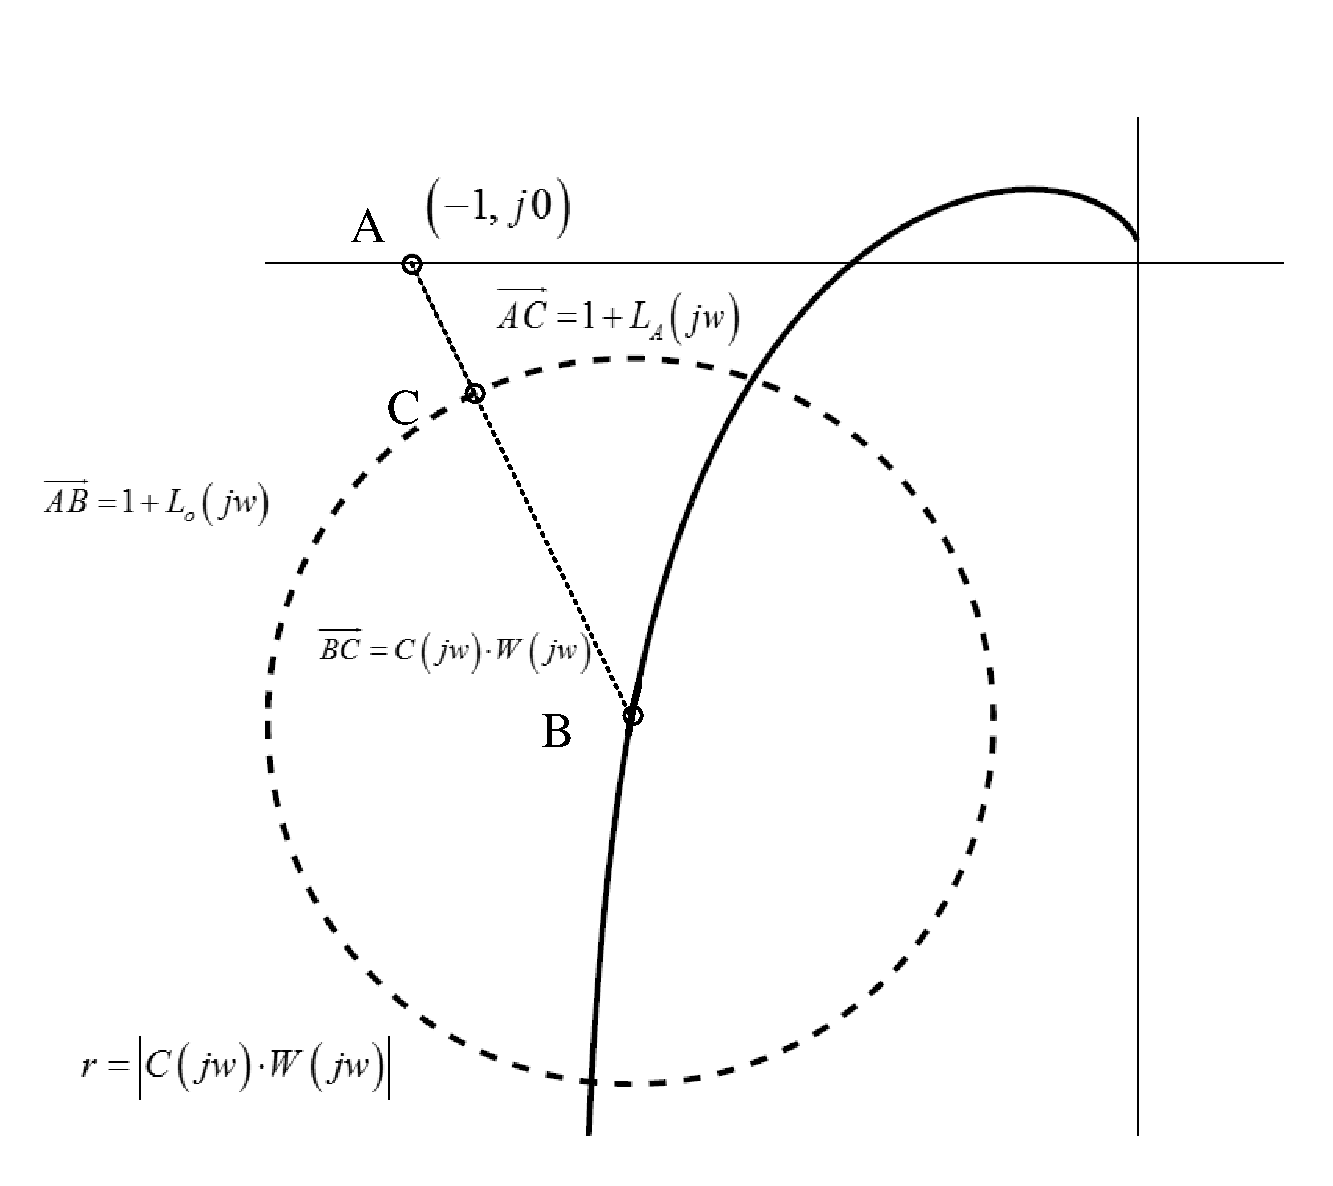
\includegraphics[width=10cm]{NyCurve2.pdf}\\
   \caption{不确定性系统最坏情况下的奈奎斯特图}\label{fig:chap3:nycurve2}
\end{figure}

经过公式推导可得
\begin{equation}\label{equ:chap3:Index25}
\left\vert\FS{\Delta P\left(jw\right)}{P\left(jw\right)}\right\vert<\left\vert\FS{1+P\left(jw\right)\cdot C\left(jw\right)}{P\left(jw\right)\cdot C\left(jw\right)}\right\vert=\FS{1}{\left\vert T\left(jw\right)\right\vert}
\end{equation}

其中~$T\left(jw\right)$~为系统补灵敏度函数的频域表达式


由于~$\left\vert\Delta P\left(jw\right)\right\vert=\left\vert\Delta\left(jw\right)\cdot W\left(jw\right)\right\vert$,取~$\left\vert\Delta \left(jw\right)\right\vert=1$~可得到
\begin{equation}\label{equ:chap3:Index26}
\left\vert\FS{W\left(jw\right)}{P\left(jw\right)}\cdot T\left(jw\right)\right\vert<1
\end{equation}

在分析系统鲁棒性时当系统满足式~\ref{equ:chap3:Index26},即该系统能够容忍加性不确定性~$\Delta P$~并在其干扰下稳定工作,则认为该控制系统对于不确定性~$\Delta P$~是鲁棒稳定的。本文中,为了进一步量化描述系统对不确定性~$\Delta P$~的容忍能力,参照控制系统稳定裕度的概念引入鲁棒稳定裕度概念。鲁棒稳定裕度~$\gamma$~的数学表达式如~\ref{equ:chap3:Index27}~式所示。相比于单纯判断系统在特定不确定性干扰下是否稳定,系统鲁棒稳定裕度概念采用量化的方式评估系统容忍特定不确定性并在其干扰下稳定工作的能力。
\begin{equation}\label{equ:chap3:Index27}
\gamma=1-\left\vert\FS{W\left(jw\right)}{P\left(jw\right)}\cdot T\left(jw\right)\right\vert_{max}
\end{equation}

由于脆弱性表征的是当系统已知部分模型参数因工作环境变化而改变时,系统容忍不确定性能力迅速变差的现象。因此由上述分析可得,在确保鲁棒裕度参数~$\gamma$~大于~0~时,研究控制系统脆弱性问题可以转化为分析控制系统在工作环境变化过程中,鲁棒稳定裕度参数~$\gamma$~的变化趋势。对系统在不同工作环境中的鲁棒稳定裕度参数进行曲线拟合,得到系统鲁棒稳定裕度变化曲线。

根据本文中脆弱性的概念,后文将围绕系统鲁棒稳定裕度变化曲线进行分析,选取能够科学有效表征曲线变化趋势的评估指标并建立合理的评估模型,对系统鲁棒稳定裕度参数~$\gamma$~的变化趋势进行量化分析,得到系统脆弱性量化评估结果。
%%%%%%%%%%%%%%%%%%%%%%%%%%%%%%%%%%%%%%%%%%%%%%%%%%%%%%%%%%%%%%%%

\section{本章小结}
\label{sec:chap3:sum}
本章节研究了控制系统稳定性、可靠性、鲁棒性等概念的具体含义以及这些控制系统性能评估指标所研究的实际问题,分析了控制系统脆弱性的本质概念,给出了本文中系统脆弱性的具体定义。由于控制系统脆弱性的产生原因是系统结构具有不确定性,本章节分析了系统不确定性的产生原因、研究了不确定性的分类并得到了控制系统在不确定性影响下的数学描述。

然后,研究控制系统性能以及反馈对负载扰动信号和测量误差扰动信号的抑制作用。结合系统灵敏度函数的概念,从奈奎斯特曲线图的角度分析控制系统在不确定性影响下的数学描述,并参照稳定裕度的概念引入评估控制系统容忍不确定性能力的鲁棒稳定裕度概念。

最后,结合本文对脆弱性概念的定义,将控制系统脆弱性问题转化为分析系统在工作环境变化过程中承受不确定性能力的变化趋势,即分析系统鲁棒稳定裕度参数的变化趋势,确定了脆弱性问题的具体研究内容,为之后建立控制系统脆弱性量化评估模型奠定了理论基础。